\documentclass[a4paper,12pt]{article}
\usepackage[utf8]{inputenc}
\usepackage[ngerman]{babel}
\usepackage[a4paper, left=2.5cm, right=2.5cm]{geometry}
\usepackage{graphicx}
\usepackage{subcaption}
\usepackage{fancyhdr}
\usepackage{pdfpages}
\usepackage{listings}
\usepackage{float}

\pagestyle{fancy}
\lstset{
	language=Matlab,
	breaklines=true,
	morekeywords={matlab2tikz},
	keywordstyle=\color{blue},
	morekeywords=[2]{1}, keywordstyle=[2]{\color{black}},
	identifierstyle=\color{black},
	stringstyle=\color{mylilas},
	commentstyle=\color{mygreen},
	showstringspaces=false,
	mathescape=true
	emph=[1]{for,end,break},emphstyle=[1]\color{red},
}

\lhead{Sonneneinstrahlung und Photovoltaik Teil 1}
\chead{}
\rhead{Gruppe D}

\begin{document}
	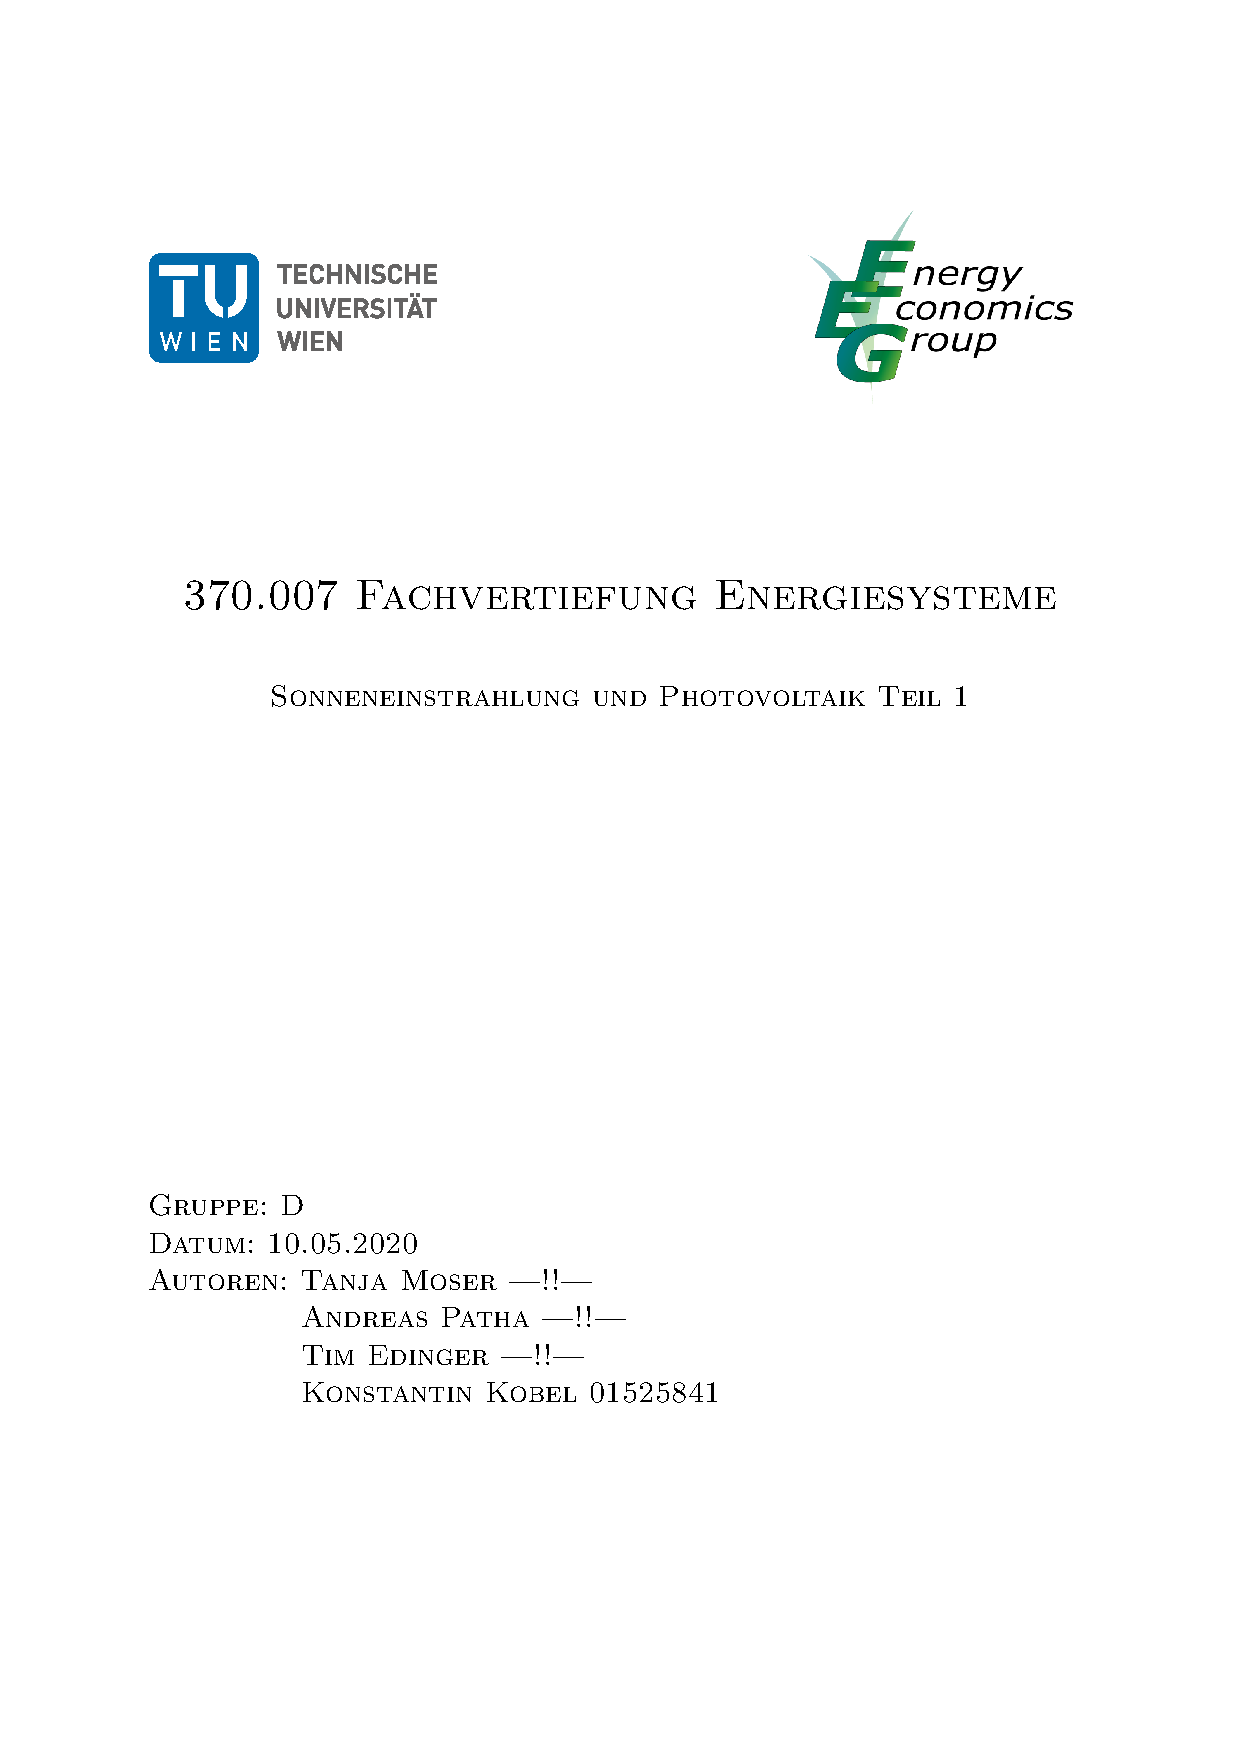
\includepdf{Protokoll_titlepage.pdf}
	
	\newpage
	%Inhaltsverzeichnis
	\tableofcontents
	
	\newpage
	\section{Aufgabenstellung}
	\subsection{Aufgabe 1.1}
	Aufgabe 1.1 befasst sich mit einer PV-Anlage mit folgenden Parametern:
	\begin{itemize}
		\item Der Standort ist Wien ($48.2^{\circ}$N, $16.3^{\circ}$O).
		\item Die installierte Leistung ist $1kWp$.
		\item Der Neigungswinkel der PV-Anlage beträgt $20^{\circ}$.
		\item Der Azimut der Anlage ist $180^{\circ}$ Süden.
		\item Der Modulwirkungsgrad $\eta_{Modul}$ ist $0.17$.
		\item Sonstige Verluste $\eta_{sonst}$ (Reflexion, Temperatur, Wechselrichter, etc.) werden mit dem Wert $0.8$ eingerechnet.
		\item Die Strahlungsdaten für den Standort sind in der Datei $Strahlung.mat$ gegeben.
		\item Die Zeit in Viertelstunden-Werten ist in der Datei $time.mat$ gegeben.
		\item Die Errechnung des Sonnenstandes erfolgt mit der in der Datei $SonnenstandTST.m$ zur Verfügung gestellten Funktion $SonnenstandTST()$.
	\end{itemize}
	Zusätzlich werden folgende Annahmen getroffen:
	\begin{itemize}
		\item Standardtestbedingungen zur Bestimmung des Modulwirkungsgrades bzw. der Nennleistung $P_{peak}$ (in W) bei $25^{\circ}$ Modultemperatur.
		\begin{equation}
			P_{peak}=R_{STC}*A*\eta_{Modul}
		\end{equation}
		\item Vereinfachte Annahme für die Bestimmung des Ertrags der Anlage im Modell.
		\begin{equation}
			E_{ges}=G_{geneigt}*A*\eta_{Modul}*\eta_{sonst}
		\end{equation}
		\item Konstanter Wirkungsgrad.
		\item Erträge bei einem Höhenwinkel unter $5^{\circ}$ werden vernachlässigt.
		\item Konstante Einstrahlung in den 15 Minuten Intervallen.
		\item Norden $5^{\circ}$, Osten $90^{\circ}$, Süden $180^{\circ}$, Westen $270^{\circ}$.
	\end{itemize}
	\newpage
	Die Aufgaben lauten:
	\begin{itemize}
		\item[a)] Erstellen Sie ein Modell, das für den gegebenen Sonnenstand und die Einstrahlungswerte (Diffus- und Direktstrahlung) auf eine horizontale Fläche den Ertrag der PV-Anlage nach Angabe der installierten Leistung in $kW_{peak}$ und der Ausrichtung der Anlage (Azimut und Neigungswinkel) modelliert. Verwenden Sie dazu das isotrope Einstrahlungsmodell.
		\item[b)] Berechnen Sie mit Hilfe der Funktion aus a) den gesamten Jahresertrag 2005 und die Volllaststunden einer $1kWp$ Anlage in Wien.
	\end{itemize}
	\subsection{Aufgabe 1.2}
	Die Unterpunkte der Aufgabe 1.2 lauten:
	\begin{itemize}
		\item[a)] Erstellen Sie die Leistungsdauerlinie der PV-Erzeugung über das Jahr. Sortieren Sie dazu die erzeugte Leistung vom Maximum bis zum Minimum.
		\item[b)] Plotten Sie die monatlichen Erträge der PV-Erzeugung (12 Werte).
		\item[c)] Ermitteln Sie jeweils die 5 Tage mit der minimalen und der maximalen PV-Erzeugung. Geben Sie die Tage (Datum) und den energetischen Ertrag dieser Tage an.
		\item[d)] Stellen Sie in einem Diagramm die Anteile der Diffus-, Direkt- und der reflektierten Strahlung an jedem der 365 Tage dar (verwenden Sie dazu das File $plotStrahlungsanteile.m$).
		\item[e)] Berechnen Sie die durchschnittliche Stromproduktion für jede Stunde am Tag für die Monate Juni und Dezember. Erstellen Sie ein Diagramm mit Boxplots der Erzeugung für jede Stunde des Tages für die jeweiligen Monate.
		\begin{itemize}
			\item Jeder Stundenwert besteht aus der Summe von vier Viertelstundenwerten.
			\item Jeder Monat wird durch eine Matrix mit den Abmessungen $Stunden x Tage$ dargestellt.
			\item Der Input eines Boxplots ist eine Matrix.
		\end{itemize}
	\end{itemize}
	\newpage
	\section{Berechnungen - Aufgabe 1.1}
	\subsection{Beschreibung der Winkel}
	\begin{figure}[H]
		\centering
		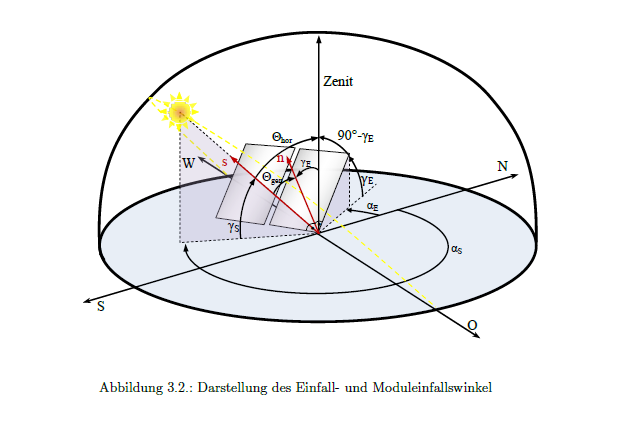
\includegraphics[width=12cm]{img/Winkel}
		\caption{Darstellung des Einfalls- und Moduleinfallswinkels.}
	\end{figure}
	\begin{itemize}
		\item $\alpha_S$ - \textbf{Sonnenazimut}. Der Sonnenazimut ist der Winkel zwischen der geographischen Nordrichtung und dem Vertikalkreis durch den Sonnenmittelpunkt. Er ist abhängig von der geographischen Breite des Standorts, der Jahreszeit und der Tageszeit.
		\item $\gamma_S$ - \textbf{Sonnenhöhe}. Die Sonnenhöhe ist der Winkel zwischen dem Sonnenmittelpunkt und der Horizontalebene vom Beobachter. Er ist ebenfalls abhängig von der geographischen Breite des Standorts, der Jahreszeit und der Tageszeit. 
		\item $\alpha_E$ - \textbf{Modulazimut}. Der Modulazimut ist der Winkel der die Modulausrichtung gegenüber dem geographischen Nordpol angibt.
		\item $\gamma_E$ - \textbf{Modulneigungswinkel.}
		\item $\Theta_{gen}$ - \textbf{Moduleinfallswinkel geneigt}. Der Einfallswinkel der Sonnenstrahlung auf eine geneigte Fläche.
		\item $\Theta_{hor}$ - \textbf{Moduleinfallswinkel horizontal}. Der Einfallswinkel der Sonnenstrahlung in horizontaler Richtung.
		\item $Zenit$ - \textbf{Zenit}. Der Zenit steht normal auf den "Horizont".
	\end{itemize}
	\subsection{Berechnung des Moduleinfallswinkels $\Theta_{gen}$}
	Der Moduleinfallswinkel $\Theta_{gen}$ ist für die Berechnung der einzelnen Strahlungsanteile relevant. Er ist von der Südausrichtung des Moduls abhängig.\\
	In unserem Fall beträgt die Südausrichtung $180^{\circ}$. Daraus folgt die Formel zur Berechnung des Moduleinfallswinkels zu
	\begin{equation}
		\Theta_{gen} = \arccos{[-\cos{(\gamma_S)}*\sin{(\gamma_E)}*\cos{(\alpha_S-\alpha_E-180^{\circ})}+\sin{(\gamma_S)}*\cos{(\gamma_E)}]}
	\end{equation}
	Der MATLAB Code, zur Berechnung des Moduleinfallswinkels $Theta_{gen}$ auf eine geneigte Fläche lautet wie folgt:
	\begin{lstlisting}
		acosd($-$cosd(sHoehenwinkel).*sind(pvHoehenwinkel).*cosd(sAzimut $-$ pvAzimut $-$ 180)+sind(sHoehenwinkel).*cosd(pvHoehenwinkel));
	\end{lstlisting}
	In dieser Formel ist hervor zu heben, dass zur Berechnung jeweils die Funktionen sind, cosd und acosd genutzt wurden. Die Besonderheit liegt darin, dass diese Funktionen den Übergabeparameter in Grad erwarten, wohingegen sin, cos und acos den Winkel in Radiant erwarten.\newline
	In der Funktion werden folgende Variablen genutzt:
	\begin{itemize}
		\item \textbf{sAzimut} - Der Sonnenazimutalwinkel der Sonne. Dieser Wert wird mit Hilfe der Funktion SonnenstandTST berechnet.
		\item \textbf{sHoehenwinkel} - Der Höhenwinkel der Sonne. Dieser Wert wird mit Hilfe der Funktion SonnenstandTST berechnet.
		\item \textbf{pvAzimut} - Der Azimutalwinkel der PV-Anlage. In unserem Fall entspricht $\alpha_E$ einem Winkel von $270^{\circ}$.
		\item \textbf{pvHoehenwinkel} - Der Höhenwinkel der PV-Anlage. Dieser entspricht dem Modulneigungswinkel. In unserem Fall entspricht $\gamma_E$ einem Winkel von $20^{\circ}$.
	\end{itemize}
	\subsection{Berechnung der Strahlungsanteile auf eine geneigte Fläche}
	Im Falle einer geneigten PV-Anlage sind drei Strahlungsanteile relevant: direkte Strahlung, diffuse Strahlung und reflektierte Strahlung. (Im Falle einer horizontalen PV-Anlage würden sich die Strahlungsanteile auf die direkte und die diffuse Strahlung begrenzen, da die reflektierte Strahlung über $\frac{1-\cos{(\gamma_E)}}{2}$ vom Modulneigungswinkel abhängig ist. Im Falle eines Modulneigungswinkels ergibt sich somit für die reflektierte Strahlung ein Wert von $0$.)
	\subsubsection{Direkte Strahlung}
	Die direkte Strahlung ist der Anteil, der direkt auf der PV-Anlage auftrifft.\newline
	Die Berechnung des direkten Strahlungsanteils erfolgt über die Formel
	\begin{equation}
		E_{dir,gen}=E_{dir,hor}*{max(0,\frac{\cos{\Theta_{gen}}}{\sin{\gamma_S}})}.
	\end{equation}
	$E_{dir,hor}$ entspricht dabei der gemessenen Direktstrahlung auf eine horizontale Fläche. Die Daten für $E_{dir,hor}$ sind in der Datei $Strahlung.mat$ gegeben.
	Der MATLAB Code für die Berechnung lautet
	\begin{lstlisting}
	DirectGen = Strahlung.DirectHoriz.*max(0, (cosd(pvModuleinfallswinkel)./sind(sHoehenwinkel)));
	\end{lstlisting}
	\subsubsection{Diffuse Strahlung}
	Der diffuse Strahlungsanteil entspricht der Strahlung, die am Weg durch die Erdatmosphäre mit ihr wechselwirkt (z.B. mit Wolken).
	Die diffuse Strahlung kann als eine Hohlhalbkugel betrachtet werden, die sich über der PV-Anlage befindet und Licht emittiert. (Isotropes Diffusstrahlungsmodell)\newline
	Die Berechnung des diffusen Strahlungsanteils erfolgt über die Formel
	\begin{equation}
		E_{diff,gen,iso}=E_{diff,hor}*\frac{1+\cos{(\gamma_E)}}{2}.
	\end{equation}
	Daraus ergibt sich folgender MATLAB Code:
	\begin{lstlisting}
	DiffusGen = Strahlung.DiffusHoriz.*(1+cosd(pvHoehenwinkel))./2;
	\end{lstlisting}
	\subsubsection{Reflektierte Strahlung}
	Bei der reflektierten Strahlung handelt es sich um den Strahlungsanteil, der zuerst vom Boden reflektiert wird und dann auf dem PV Modul auftrifft.\newline
	Daraus folgt die Formel zur Berechnung des reflektierten Strahlungsanteils zu
	\begin{equation}
		E_{refl,gen}=E_{G,hor}*A*\frac{1-\cos{(\gamma_E)}}{2}.
	\end{equation}
	$A$ entspricht in dieser Formel dem Albedo-Wert. Dieser entspricht dem Verhältnis der auf eine Fläche einfallenden Strahlung und der von der Fläche reflektierten Strahlung. Ist dieser Wert für eine Fläche nicht bekannt, kann er mit dem Wert $0.2$ angenommen werden.\newline
	Der daraus resultierende MATLAB Code, zur Errechnung der reflektierten Strahlung, lautet
	\begin{lstlisting}
	ReflectedGen = Strahlung.Reflected.*0.2.*(1$-$cosd(pvHoehenwinkel))./2;
	\end{lstlisting}
	\subsection{Berechnung der gesamten Strahlung auf eine geneigte Fläche}
	Wie bereits eingangs erwähnt, setzt sich die gesamte Strahlung auf eine geneigte Fläche aus dem direkten, dem diffusen und dem reflektierten Strahlungsanteil zusammen.\newline
	Daraus ergibt sich
	\begin{equation}
		E_{G,gen}=E_{dir,gen}+E_{diff,gen,iso}+E_{refl,gen}.
	\end{equation}
	Unter Berücksichtigung des obigen MATLAB Codes ergibt sich für die Berechnung der gesamten Strahlung auf eine geneigte Fläche
	\begin{lstlisting}
	GesGen = DirectGen + ReflectedGen + DiffusGen;
	\end{lstlisting}
	Als zusätzliche Annahme wurde definiert, dass Erträge bei einem Höhenwinkel unter $5^{\circ}$ nicht berücksichtigt werden sollen.\newline
	Diese Annahme lässt sich durch folgende Formel umsetzen:
	\begin{lstlisting}
	GesGen(sHoehenwinkel < 5) = 0;
	\end{lstlisting}
	\subsection{Berechnung des Ertrags}
	Der gesamte Ertrag $E_{ges}$ der Anlage errechnet sich durch
	\begin{equation}
		E=E_{G,gen}*A*\eta_{Modul}*\eta_{sonst}.
	\end{equation}
	\begin{itemize}
		\item \textbf{$E_{G,gen}$} entspricht der gesamten Einstrahlung (dem gesamten Ertrag) auf die geneigte PV-Anlage.
		\item \textbf{$A$} entspricht der Fläche der PV-Anlage.
		\item \textbf{$\eta_{Modul}$} ist der Modulwirkungsgrad (in unserem Fall $0.17$).
		\item \textbf{$\eta_{sonst}$} sind sonstige Verluste, die durch Reflexion, die Temperatur, Wechselrichter, etc. auftreten. (In unserem Fall $0.8$).
	\end{itemize}
	Da die in der Variable $E_{G,gen}$ errechneten Werte in 15 Minuten Intervalle aufgeteilt sind, müssen wir in MATLAB eine zusätzliche Korrektur (ein Multiplikator mit dem Wert $0.25$) in die Formel einfügen:
	\begin{lstlisting}
		Eges = GesGen.*0.25.*pvFlaeche.*pvWirkungsgrad.*pvVerluste;
	\end{lstlisting}
	\newpage
	\section{Ergebnisse - Aufgabe 1.1}
	\subsection{1.1.a}
	In Aufgabe 1.1.a ging es darum ein Modell zu erstellen, das für eine bestimmte Anlage (mit gegebenem Sonnenstand und Einstrahlungswerten) den Ertrag der PV-Anlage errechnet.\newline
	Das Modell zur Berechnung des Ertrags befindet sich in der Datei $Beispiel1.m$. Die Ergebnisse der Berechnungen werden im Unterpunkt 1.1.b beschrieben.
	\subsection{1.1.b}
	In Aufgabe 1.1.b waren der gesamte Jahresertrag 2005 und die Volllaststunden, der in der Angabe parametrisierten Anlage, zu errechnen.\newline
	Die Ergebnisse der Berechnungen befinden sich in den Dateien $Jahresertrag\_2005.mat$ beziehungszweise $Vollaststunden.mat$.\newline
	Durch Aufsummieren der einzelnen Viertelstunden-Erträge, erhält man für das Jahr 2005 einen Gesamtertrag von $219.25kWh$.\newline
	Über die Formel
	\begin{equation}
	T=\frac{\sum \limits_{t=1}^T P_t}{P_{Peak}}
	\end{equation}
	können die Volllaststunden der Anlage errechnet werden. Im Falle unserer $1kWp$ Anlage ergibt sich eine Vollauslastung von etwa $219.25$ Stunden.
	\begin{figure}[H]
		\centering
		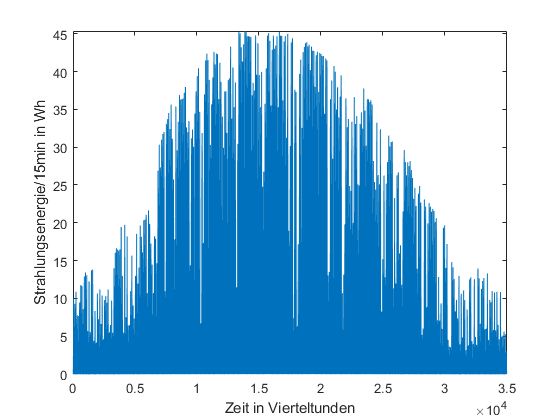
\includegraphics[width=12cm]{img/results/Gesamtertrag}
		\caption{Gesamtertrag der PV-Anlage, über das Jahr 2005.}
	\end{figure}
	\section{Ergebnisse - Aufgabe 1.2}
	\subsection{1.2.a - Leistungsdauerlinie}
	Das Ziel der Aufgabe 1.2.a war eine Leistungsdauerlinie der PV-Erzeugung, über das Jahr, darzustellen.\newline
	Eine Leistungsdauerlinie gibt die erbrachte Leistung der PV-Anlage, über eine bestimmte Zeitspanne, an.\newline
	Die Leistung $P$ der Anlage ergibt sich aus
	\begin{equation}
	P=E*15
	\end{equation}
	Die Mulitplikation mit $15$ ist nötig, da die Energie der Anlage mit $Wh/15min$ gegeben ist.\newline
	Um aus dem berechneten gesamten Ertrag der PV-Anlage die Leistungsdauerlinie zu erhalten, ist folgender MATLAB Code notwendig:
	\begin{lstlisting}
	sort(Eges, $'$descend$'$).*15;
	\end{lstlisting}
	\newpage
	Daraus ergibt sich folgendes Diagramm:
	\begin{figure}[H]
		\centering
		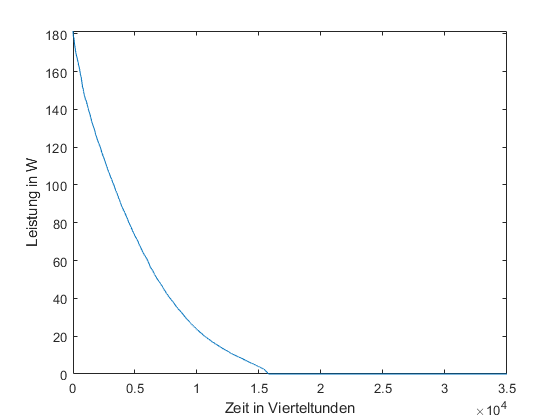
\includegraphics[width=12cm]{img/results/Leistungsdauerlinie}
		\caption{Leistungsdauerlinie der PV-Anlage, im Jahre 2005. (x-Achse in Viertelstunden-Schritten)}
	\end{figure}
	In Abbildung 2 ist ersichtlich, dass die PV-Anlage in einem Zeitraum von ungefähr $5.2$ Monaten ($\sim 16.000$ Viertelstunden) Energie liefert. Der Grund, warum die Anlage die restlichen $6.8$ Monate keine Energie liefert, ist einerseits die Nacht. Andererseits ist die Anlage nicht nachgeführt, was zu einem geringeren Ertrag in den Morgen- und Abendstunden führt.
	\subsection{1.2.b - monatliche Erträge}
	In Aufgabe 1.2.b ging es darum einen Plot über die monatlichen Erträge der PV-Anlage zu erstellen.\newline
	Der Plot kann mit folgendem MATLAB Code erstellt werden:
	\begin{lstlisting}
	plot(Eges);
	\end{lstlisting}
	\begin{figure}[H]
		\centering
		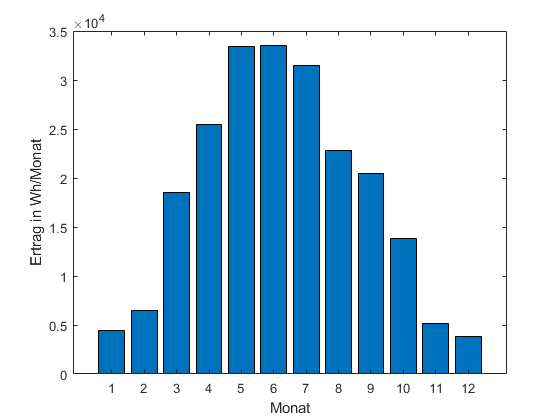
\includegraphics[width=12cm]{img/results/MonatlicheErtraege}
		\caption{Monatliche Erträge der PV-Anlage, über das Jahr 2005.}
	\end{figure}
	In Abbildung 3 ist schön dargestellt, wie der Ertrag der PV-Anlage in den Sommermonaten deutlich höher ist, als in den Wintermonaten.\newline
	Das ist dadurch begründet, dass in den Sommermonaten die Strahlungsleistung auf einen Quadratmeter deutlich höher ist und die Tage zusätzlich länger sind, als in den Wintermonaten.\newline
	Da wir in der Angabe definiert haben, dass der Wirkungsgrad der PV-Anlage konstant ist, wurde der Faktor "Temperatur" nicht in der Berechnung berücksichtigt.\newline
	Dieser würde jedoch dafür sorgen, dass der Wirkungsgrad bei höheren Temperaturen sinkt und bei niedrigeren Temperaturen steigt.
	\subsection{1.2.c - Ertragsminima und Ertragsmaxima}
	Das Ziel von Aufgabe 1.2.c war es jeweils die fünf ertragreichsten und ertragsschwächsten Tage zu identifizieren.\newline
	Hierzu müssen die Viertelstunden-Erträge in der Variable $Eges$ zuerst zu ganzen Tagen aufsummiert werden.
	\newpage
	Dies geschieht über folgenden Code:
	\begin{lstlisting}
	Etag = zeros(1,365);
	for tag=1:365
		Etag(tag) = sum(Eges(time.Tag == tag));
	end
	\end{lstlisting}
	Um nun die fünf ertragsstärksten bzw. ertragsschwächsten Tage zu ermitteln, können die Funktionen $maxk(Etag, 5)$ bzw. $mink(Etag, 5)$ benutzt werden.\newline
	Daraus ergeben sich für die ertragsstärksten Tage:
	\begin{table}[H]
		\begin{tabular}{|c|c|c|c|c|c|}
			\hline
			Tagesertrag (in Wh) & 1.5104e+03  & 1.5079e+03  & 1.4992e+03  & 1.4989e+03  & 1.48783+03  \\ \hline
			Datum               & 21-Jun-2005 & 24-Jun-2005 & 23-Jun-2005 & 03-Jun-2005 & 04-Jul-2005 \\ \hline
		\end{tabular}
	\end{table}
	\noindent Die ertragsschwächsten Tage sind:
	\begin{table}[H]
		\begin{tabular}{|c|c|c|c|c|c|}
			\hline
			Tagesertrag (in Wh) & 52.7921     & 54.5420     & 58.0446     & 59.8388     & 60.2442     \\ \hline
			Datum               & 06-Dec-2005 & 31-Dec-2005 & 27-Nov-2005 & 03-Dec-2005 & 28-Dec-2005 \\ \hline
		\end{tabular}
	\end{table}
	\noindent Die ertragsstärksten Tage liegen, wie erwartet, in den Sommermonaten (in diesem Fall alle im Juni), während die ertragsschwächsten Tage in den Wintermonaten (in unserem Fall Dezember) liegen.\newline
	Die PV-Anlage produziert maximal $1.5104e+03Wh$ und minimal $52.7921Wh$. Die Verteilung über jeweils einen Tag ist glockenförmig, mit einem Maximum bei circa 12:00 Uhr.
	\subsection{1.2.d - Strahlungsanteile}
	Zur Darstellung der Strahlungsanteile in einem Diagramm, steht uns die Funktion $plotStrahlungsanteile.m$ zur Verfügung.\newline
	Damit ergibt sich folgender MATLAB Code:
	\begin{lstlisting}
	plotStrahlungsanteile(pvAzimut, pvHoehenwinkel, sLaengengrad, sBreitengrad, Strahlung, time)
	\end{lstlisting}
	Das resultierende Diagramm ist in Abbildung 4 dargestellt.
	\begin{figure}[H]
		\centering
		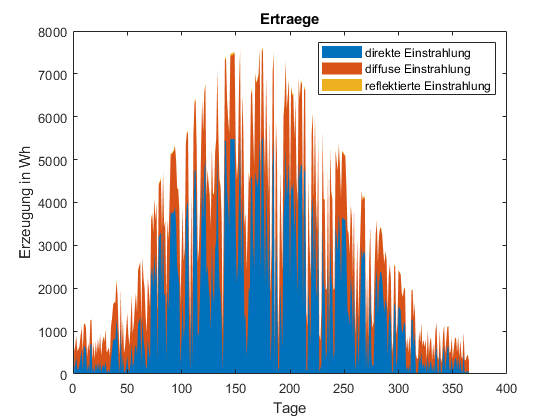
\includegraphics[width=12cm]{img/results/Strahlungsanteile}
		\caption{Strahlungsanteile, über das Jahr 2005.}
	\end{figure}
	Wie erwartet kommt der Großteil der Strahlungsenergie von der direkten und der diffusen Strahlung. Der reflektierte Anteil trägt relativ wenig zur Energie bei.
	\subsection{1.2.e - Durchschnittliche Stromproduktion}
	In Aufgabe 1.2.e sollte die durchschnittliche Stromproduktion für jede Stunde am Tag, für die Monate Juni und Dezember, berechnet werden. Die Darstellung soll mithilfe von Boxplots geschehen.\newline
	Mithilfe folgendem MATLAB Code erhalten wir eine $24 x 30$ Matrix, die uns zu jedem Tag des Monats Juni den Ertrag in $Wh$ angibt:
	\begin{lstlisting}
	Ejuni = Eges(time.Monat == 6);
	EJuniStunden = sum(reshape(Ejuni,4,720));
	EJuniTage = reshape(EJuniStunden,24,30);
	\end{lstlisting}
	Analog dazu kann die Matrix für Dezember folgendermaßen errechnet werden:
	\begin{lstlisting}
	Edezember = Eges(time.Monat == 12);
	EDezemberStunden = sum(reshape(Edezember,4,744));
	EDezemberTage = reshape(EDezemberStunden,24,31);
	\end{lstlisting}
	\newpage
	Die resultierenden Boxplot Diagramme sehen folgendermaßen aus:
	\begin{figure}[H]
		\centering
		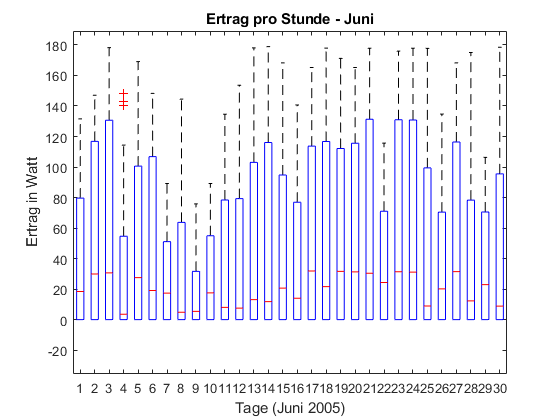
\includegraphics[width=12cm]{img/results/ErtragProStunde_Juni}
		\caption{Ertrag pro Stunde, über das Monat Juni 2005.}
	\end{figure}
	\begin{figure}[H]
		\centering
		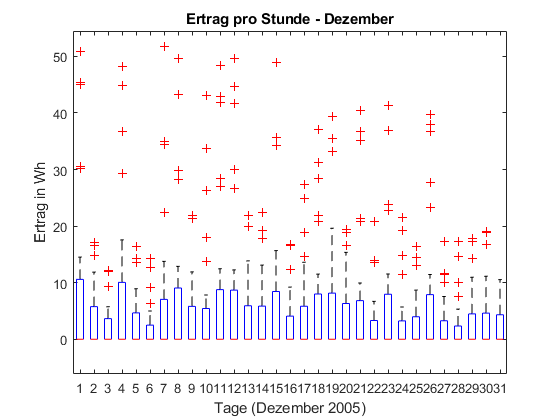
\includegraphics[width=12cm]{img/results/ErtragProStunde_Dezember}
		\caption{Ertrag pro Stunde, über das Monat Dezember 2005.}
	\end{figure}
	\section{Interpretation der Ergebnisse}
	Die errechneten Werte basieren auf Annahmen, die unter Anderem einen, durch die Tempertatur veränderten, Wirkungsgrad der PV-Anlage, Verschattung durch Bäume und Gebäude und Verschmutzung nicht berücksichtigen. Sie vermitteln daher eine ungefähre Idee über den Ertrag der Anlage, sollten jedoch nur in Anbetracht dieser Annahmen weiterverwendet werden.
	\section{Literatur}
	Modellierung eines Wärmeschichtspeichers mit
	Solareinbindung in Excel/VBA von Rainer Blabensteiner.
\end{document}